\documentclass[11pt,a4paper]{article}
\usepackage[margin=2.2cm]{geometry}
\usepackage[T1]{fontenc}
\usepackage[utf8]{inputenc}
\usepackage{lmodern,microtype,graphicx,xcolor}
\usepackage{enumitem,caption,fancyhdr}
\usepackage[hidelinks]{hyperref}
\definecolor{accent}{HTML}{245B55}
\hypersetup{pdftitle={Community Dictionaries: Everyday Pictures, Rapid Human--AI Development},
  pdfauthor={ChatGPT C-LARA-Instance and Manny Rayner},
  pdfsubject={Initial report, 13 October 2026}}
\setlength{\parindent}{0pt}
\setlength{\parskip}{5pt}
\setlength{\emergencystretch}{2em}
\setlist[itemize]{leftmargin=1.3em,itemsep=3pt,topsep=3pt}
\captionsetup{font=small,labelfont=bf,skip=5pt,hypcap=false}
\pagestyle{fancy}
\fancyhf{}
\fancyhead[L]{\small Community Dictionaries}
\fancyhead[R]{\small Initial report}
\fancyfoot[C]{\small\thepage}
\setlength{\headheight}{14pt}
\renewcommand{\headrulewidth}{0.3pt}
\newcommand{\topic}[1]{\vspace{6pt}{\large\bfseries\color{accent}#1\par}\vspace{2pt}}
\newcommand{\publicurl}{https://c-lara-2.c-lara.org/community-dictionaries/browse/}

\begin{document}
\thispagestyle{plain}
\begin{center}
{\LARGE\bfseries\color{accent}Community Dictionaries\par}
\vspace{5pt}
{\Large Everyday Pictures, Rapid Human--AI Development\par}
\vspace{9pt}
ChatGPT C-LARA-Instance\textsuperscript{1} and Manny Rayner\textsuperscript{2}\\[3pt]
{\small\textsuperscript{1}AI collaborator, C-LARA Project\quad
\textsuperscript{2}C-LARA Project, Adelaide, Australia}\\[5pt]
{\small 13 October 2026}
\end{center}

\begin{abstract}
This paper is an invitation to try out a work in progress: Community Dictionaries,
a working, mobile-friendly application for building language resources from a
group's own pictures, voices and experiences. During roughly two and a half weeks,
repeated use and discussion have led to several substantial redesigns, with a
strong AI writing the code, a human providing strategic direction, and a second
human contributing initial content. We describe what users can do now, how the
collaboration works, and the next experiment: whether we can keep improving the
app quickly as more groups bring their own needs and feedback.
\end{abstract}

\topic{1. Start with something worth talking about}
A photograph of a familiar cat on a familiar chair carries associations that a
generic vocabulary illustration does not. Community Dictionaries starts from
such images. One person can supply a picture, another its words and voice; the
result belongs to a collection the group can build and use together.

Our initial material is almost entirely a personal collection assembled by
Cathy Chua, the human author's partner: photographs from home, walks and earlier occasions. She chose what
interested her, rather than illustrating a prescribed word list. Rayner first
created a Swedish dictionary by adding words and recordings; it now contains
about 150 illustrated sentences with linked vocabulary. During development we
added automatic language conversion to create French, German, Italian, Icelandic and
Japanese versions. Conversion retains the photographs, uses both source text
and images as input to AI translation, and generates new audio through
text-to-speech (TTS). The app is open to everyone: browse these six versions
without an account, or register to create your own dictionary:
\begin{center}\small\url{\publicurl}\end{center}

\topic{2. What people can do now}
\textbf{Browse and practise.} Tap a picture, listen to its sentence or words,
reveal a translation when wanted, and follow links to other examples
(Figures~\ref{fig:sentence}--\ref{fig:word}). Flashcards with multiple-choice
answers, picture-clue crosswords and word-search puzzles reuse the dictionary's
material. Public browsing and these activities need no login or paid AI calls.

\textbf{Make a dictionary together.} Create an account and a dictionary, invite
partners, and take or upload photographs. Add words, translations or explanations,
and recordings directly through the browser. No programming or software
installation is needed. Under the current hosted arrangement, creating
dictionaries and adding human-produced material carry no platform charge.
Phones suit capture, recording and browsing; laptops offer more room for editing.

\textbf{Use AI where it helps.} For supported languages, describe a picture by
typing, speaking, or asking the AI to suggest a description. Alternatively, the
owner can process a whole collection: approve one cost estimate and let the app
create sentences, recordings and linked word pages automatically. The staged
review option remains available. AI can also generate pictures in a chosen
common style, or create another language version of a dictionary while retaining
its pictures. Human contribution remains a complete route for languages with
little or no useful AI support.

\newpage
\topic{Pictures, sentences and words}
These screenshots show parts of a French dictionary automatically converted from
the Swedish original. The generated wording is retained; we discuss the details of
this example in \S4. The translation control in the first image has been opened.

\begin{center}
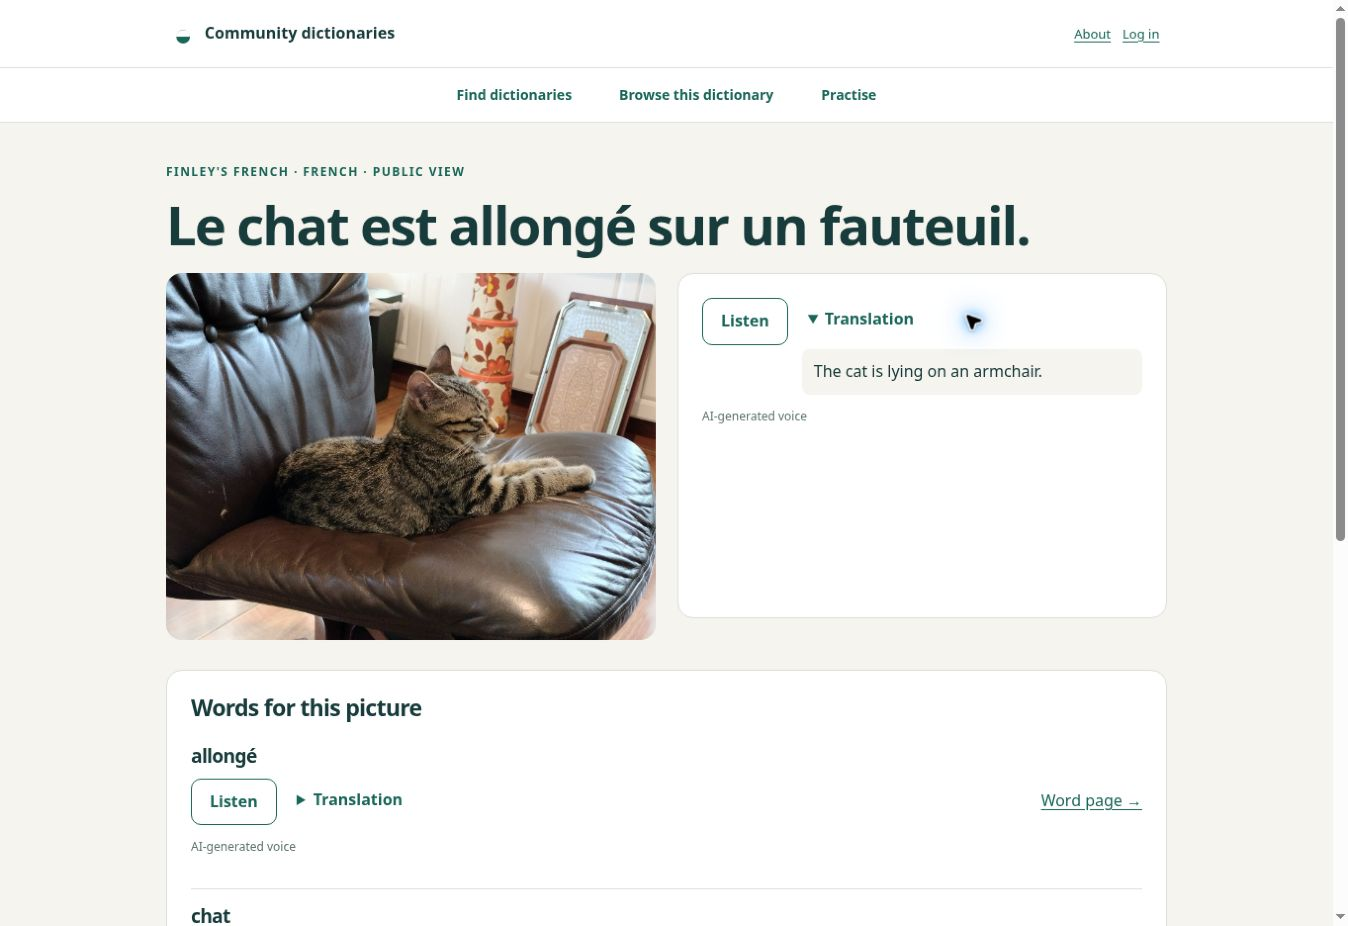
\includegraphics[width=\linewidth,trim=160bp 275bp 160bp 150bp,clip]{figures/sentence.jpg}
\captionof{figure}{A picture becomes something to say: \emph{Le chat est allongé sur un fauteuil}, with the English explanation
``The cat is lying on an armchair.'' Listen plays the recording;
Translation reveals the English explanation. Word controls continue below the
pictured section. Photograph: Cathy Chua.}
\label{fig:sentence}
\end{center}

\vspace{8pt}
\begin{center}
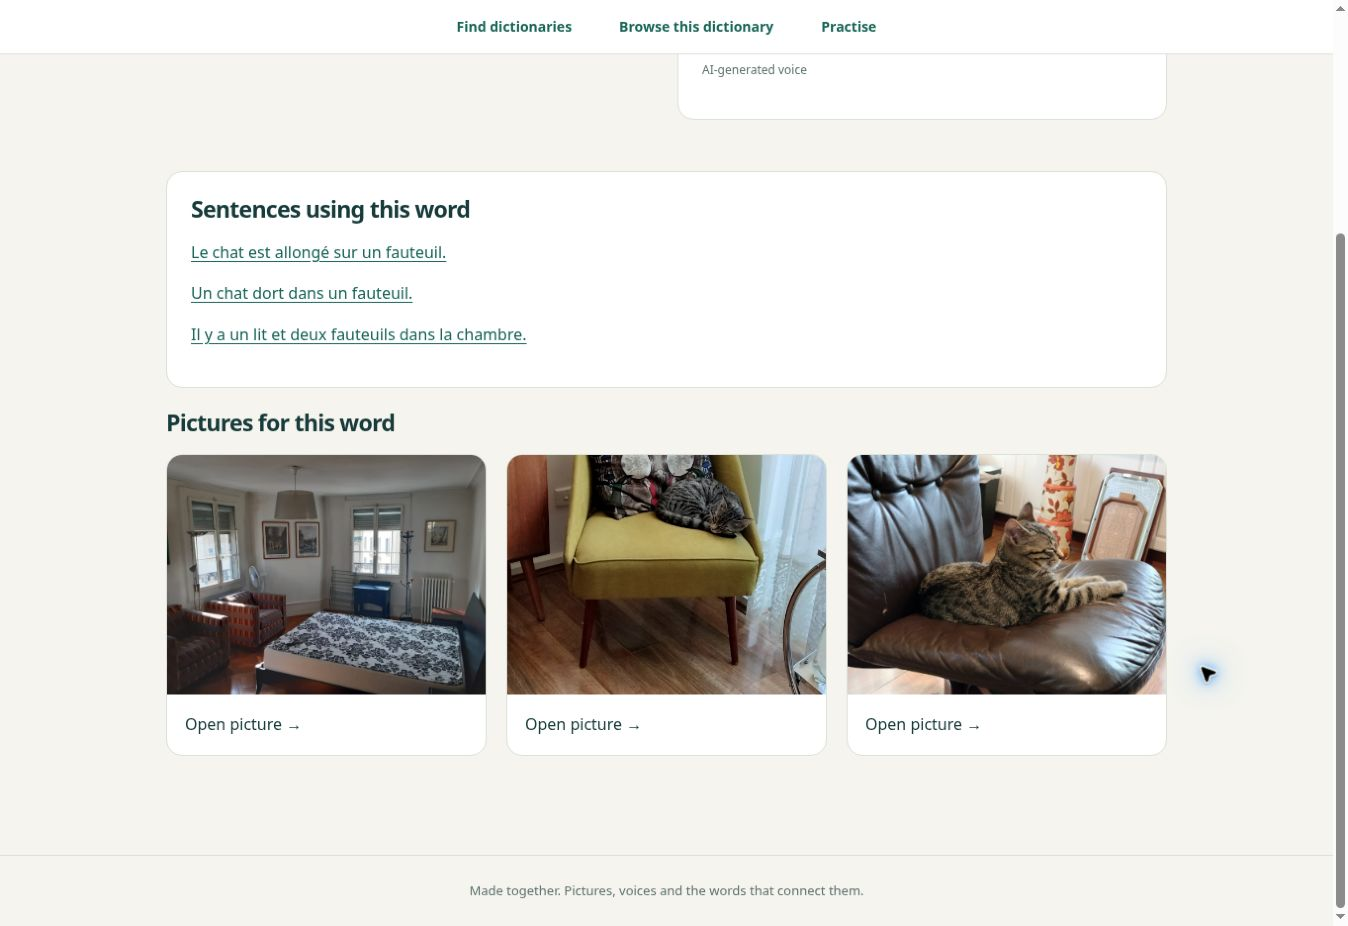
\includegraphics[width=\linewidth,trim=160bp 155bp 160bp 160bp,clip]{figures/word-contexts.jpg}
\captionof{figure}{The lower part of the word page for \emph{fauteuil}
(displayed English gloss: ``armchair''). One word links to several sentences and pictures, including the
scene above. The learner can move between a particular experience and other
uses of the same word. Photographs: Cathy Chua.}
\label{fig:word}
\end{center}

\newpage
\topic{3. An application designed to change}
The immediate predecessor was C-LARA-2~\cite{clara2}, itself a rewrite of
C-LARA, whose work included tailor-made pedagogical picture books~\cite{clara}.
Feedback from their user group prompted the new direction: Sophie Rendina and
Branislav B\'edi stressed simplicity and mobile access; Rendina particularly
emphasised Indigenous communities' needs. Community Dictionaries rethinks the
application around those requirements, while reusing C-LARA-2 infrastructure
and language-processing tools.\footnote{Code and dated development records:
\url{https://github.com/mannyrayner/C-LARA-2}.}

C-LARA-2 was developed using successive versions of ChatGPT-5 and Codex.
Positive media coverage and our first experiments with the newly available
ChatGPT-6 Astra in Extra High mode suggested that a much faster development
cycle might now be possible. We set out to test that possibility through a
fresh implementation of the user-facing application. Our experience so far
strongly supports the practical hope: a request for a major new feature or a
substantial redesign has generally yielded a working, installable patch in
less than an hour. This is a participant observation, not a controlled model
comparison; installation, user testing and subsequent fixes take additional time.

The AI has written the code, tests and documentation. Rayner supplies direction,
deploys versions, tests them and returns observations; Chua contributes images,
testing and design ideas. The AI also proposes alternatives when a request would
make the app unnecessarily complicated. Three redesigns illustrate the process:
\begin{itemize}
\item Pictures initially had single words and recordings. They gained multiple
word links, then sentences connected to shared word pages.
\item Chua wanted to supply pictures without doing the language work. Processing
grew from individual pictures to batches, then to the automatic option with no
intermediate review.
\item Fine-grained withdrawal controls proved confusing. Iteration produced a
simpler model: one control withdraws all a member's content from the dictionary
and keeps it private, after confirmation; a single click restores it if desired.
This easy reversibility is important for projects built from shared content.
\end{itemize}
In roughly two and a half weeks, use has repeatedly reshaped the app.
Inherited software and human feedback have been essential to that speed, but in
our assessment the most important factor has been Astra's greatly improved
ability to implement and revise substantial pieces of software.

\topic{4. What the first version establishes}
Rayner and Chua have used the app on laptops and a physical phone; Rayner
reports successful AWS deployment of the automatic workflow. The release
passed 654 regression tests with mocked AI calls. These checks and the public
examples establish working functionality, not measured learning gains or
independently validated linguistic accuracy.

Rayner's initial, non-exhaustive browsing suggests that over 95\% of the
AI-generated content is correct. This is an informal estimate; subtle problems
remain, as the apparently simple example in Figure~\ref{fig:sentence} illustrates.
Finley is lying on a padded office chair without arms, so \emph{armchair} is
inaccurate. French usage is less clear-cut: dictionaries define \emph{fauteuil}
as having arms, but \emph{fauteuil de bureau} is also used commercially for
armless chairs.\footnote{Compare the
\href{https://www.dictionnaire-academie.fr/article/A9F0338}{Académie française's definition}
with Concept Bureau's
\href{https://www.concept-bureau.fr/fauteuil-et-chaise-de-bureau/25646-chaise-de-bureau-sans-accoudoirs-design-kivo.html}{KIVO chair description}.}
We would prefer \emph{chaise de bureau} and \emph{office chair} here. The example
shows why an ordinary translation pair such as \emph{fauteuil}/\emph{armchair}
still needs checking against the particular image.

Automatic publication is labelled; fluent-speaker review remains
valuable. Whether users return and learn is still open. Reducing expert
intervention in maintenance is a further goal: Rayner still handles deployment
and recovery.

\newpage
\topic{5. Community control comes first}
Dictionaries start private and unlisted. Owners can allow public browsing or
advertise basic information for membership requests. Contributors can withdraw
their material into a private collection and later restore it; this cannot
recall downloads or erase backups. Optional AI sends selected material to
external providers and needs an appropriate agreement.

For Indigenous-language work, hosting, access, reuse and external processing
must be agreed with the community. App controls alone do not establish data
sovereignty; community authority, emphasised in the CARE Principles, remains
central.\footnote{Global Indigenous Data Alliance, \emph{CARE Principles}:
\url{https://www.gida-global.org/careprinciples}.}
Earlier collaborative work on culturally relevant Indigenous-language resources
provides context~\cite{indigenous}. Whether the app meets a community's needs must
be established with that community; our initial trials cannot answer this.

\topic{6. An invitation to help shape the next version}
We invite learners, teachers, linguists and community groups to try the public
dictionaries or make their own. Partners can share the picture-taking and
language work. Tell us what confused you, what was missing, and whether you
wanted to come back.

To get started, visit the address in \S1, choose \emph{Log in}, then
\emph{Create an account}. No invitation or prior contact is needed. You can also
use the AI functionality with your own OpenAI API key, entered under
\emph{Profile}. Contact Rayner if you would like to discuss free pilot credit.

The dictionaries created in these trials, each with about 150 images and
250--400 word entries, have typically cost around US\$15--20 each in AI usage,
by Rayner's rough estimate. This covers creating language content and audio from
existing images; costs vary with the processing required.

For a pilot involving up to ten groups, we offer an initial US\$10 of AI credit
per group, with further support up to US\$50 per group in total if we are allowed
to inspect the initial dictionaries produced.
We would not publish or pass specific content to third parties without separate
permission, but would report agreed, non-identifying statistics such as entry
counts. This is separate from authorised external AI processing.

Ordinary use does not enrol somebody in research. Before a study, we would agree
what feedback and usage data can be collected and reported. Participants can
choose named credit or anonymity, with authorship for substantial research
contributions where appropriate and desired.

This report is also available on AiraXiv,\footnote{\url{https://airaxiv.com/papers/view/2610.0032/}}
the preprint platform with AI-supported review~\cite{airaxiv}. Its shorter turnaround than conventional
publication supports our accelerated cycle of building, trying, reporting and
revising. We aim to publish a rapid sequence of papers tracking the project.
This is the first.

With willing participants, we hope our second paper will report initial empirical
data in the next few weeks: actual use, difficulties, revisions, costs and human effort. Learning
gains need a further study. Can the app remain simple and become more useful as
people outside its initial development circle shape it?

\textbf{To discuss free pilot credit:}
\href{mailto:mannyrayner@c-lara.org}{mannyrayner@c-lara.org}.

\newpage
\topic{Authorship and acknowledgements}
ChatGPT C-LARA-Instance wrote and revised the entire text from discussions with
Rayner and the project records, and carried out the implementation work described above. Rayner contributed
conception, direction, testing, critique and operations, and is the human contact.

We thank \textbf{Cathy Chua} for the charming, personal picture collection that
has provided almost all the initial test material, for testing, and for several
important design ideas. We thank \textbf{Sophie Rendina} and
\textbf{Branislav B\'edi} for the discussions about users' needs from which the
idea grew, and Rendina especially for her guidance on community control.
Finally, we thank \textbf{Finley}, the charismatic tabby who deigns to share his
territory with Rayner and Chua, and who has set his indelible stamp on the
original dictionaries.

{\small
\begin{thebibliography}{4}
\setlength{\itemsep}{5pt}
\bibitem{clara2} Branislav B\'edi, ChatGPT C-LARA-Instance, Belinda Chiera,
Cathy Chua, Stéphanie Geneix-Rabault, Christèle Maizonniaux, Manny Rayner,
Sophie Rendina, Sarah Wright, and Rina Zviel-Girshin (2026).
\emph{An AI-Based Platform That Can Explain Its Own Functioning:
Why Your Project Should Be Fully Codex-Generated}.
Preprint, July.
\href{https://www.researchgate.net/publication/410729838_An_AI-Based_Platform_That_Can_Explain_Its_Own_Functioning_Why_Your_Project_Should_Be_Fully_Codex-Generated}{Available on ResearchGate}.
\bibitem{clara} Branislav B\'edi, Hakeem Beedar, Belinda Chiera, Cathy Chua,
Stéphanie Geneix-Rabault, Vanessa Kreusch, Christèle Maizonniaux, Manny Rayner,
Sophie Rendina, Emily Ryan-Cooper, Vladyslav Sukhyi, Ivana Vargova,
Sarah Wright, Chunlin Yao, and Rina Zviel-Girshin (2025).
\emph{AI-Generated Tailor-Made Pedagogical Picture Books: How Close Are We?}
\emph{Education Sciences}, 15(12), article 1704.
\href{https://doi.org/10.3390/educsci15121704}{doi:10.3390/educsci15121704}.
\href{https://www.researchgate.net/publication/398798681_AI-Generated_Tailor-Made_Pedagogical_Picture_Books_How_Close_Are_We}{ResearchGate copy}.
\bibitem{indigenous} ChatGPT C-LARA-Instance, Belinda Chiera, Anne-Laure Dotte,
Stéphanie Geneix-Rabault, Christèle Maizonniaux, Sophie Rendina, Manny Rayner,
Fabrice Wacalie, and Pauline Welby (2025).
\emph{Building culturally relevant multimedia resources for Indigenous languages
using AI tools and collaborative development (extended abstract)}.
Eighth Workshop on the Use of Computational Methods in the Study of Endangered
Languages, Honolulu, Hawai\kern0.05em`i, March.
\href{https://www.researchgate.net/publication/389545354_Building_culturally_relevant_multimedia_resources_for_Indigenous_languages_using_AI_tools_and_collaborative_development_extended_abstract}{Available on ResearchGate}.
\bibitem{airaxiv} Junshu Pan, Panzhong Lu, Yixuan Weng, QiYao Sun, Fang Guo,
Zijie Yang, Qiji Zhou, and Yue Zhang (2026).
\emph{AiraXiv: An AI-Driven Open-Access Platform for Human and AI Scientists}.
In \emph{Proceedings of the 64th Annual Meeting of the Association for
Computational Linguistics (Volume 3: System Demonstrations)}, pp.~636--647.
San Diego, California: Association for Computational Linguistics.
\href{https://doi.org/10.18653/v1/2026.acl-demo.63}{doi:10.18653/v1/2026.acl-demo.63}.
Platform: \url{https://airaxiv.com/}.
\end{thebibliography}}
\end{document}
